\documentclass[12pt, a4paper]{article}
\title{Изучение поляризованного света (4.7.3)}
\author{Стеценко Георгий, Б02-312}
\date{}
% !TeX encoding = UTF-8

\usepackage{geometry}
\usepackage{amsmath, amsfonts, amssymb, amsthm} % стандартный набор AMS-пакетов для математ. текстов
\usepackage{mathtext}
\usepackage[utf8]{inputenc} % кодировка utf8
\usepackage[russian]{babel} % русский язык
\usepackage[pdftex,dvipsnames]{xcolor} % работа с цветами
\usepackage[pdftex]{graphicx} % графика (картинки)
\usepackage{tikz,pgfplots} % рисунки
\usepackage{indentfirst}
%\usepackage[labelfont=bf,labelsep=endash,skip=3pt]{caption} % подпись картинок
% \usepackage{fancyhdr,pageslts} % настройка колонтитулов
\usepackage{enumitem} % работа со списками
\usepackage{floatrow,multicol,multirow,longtable,hhline} % работа с таблицами
\usepackage{float,wrapfig} % плавающие объекты
\usepackage{tcolorbox} % рамка вокруг текста
%\usepackage[calc]{datetime2} % дата
\usepackage{bm} % жирное начертание в формулах
\usepackage{physics} % физический пакет
\DeclareMathAlphabet\mathbfcal{OMS}{cmsy}{b}{n}
\usepackage{pgfornament} % красивые рюшечки и вензеля
\usepackage{mdframed}
\usepackage{derivative}
\usepackage{mathrsfs} %EDS
\usepackage{soul} % strikethorugh
%\usepackage{boondox-cal}

% ----------------------------------------
% Настройка шрифта

% Просто закооментируйте следующую строчку, если не работает. Будет другой шрифт, правда :(
% \usepackage{pscyr}

% ----------------------------------------
% Стилевые настройки

\usepackage{boldline} % жирная линия после таблиц (чтобы не было ошибок, этот пакет должен подключаться именно тут!)
\floatsetup[table]{style=Plaintop,floatrowsep=qquad} % настройка оформления таблиц
\setlist[enumerate,itemize]{leftmargin=5mm,itemindent=10mm,itemsep=0mm,
listparindent=0em,labelsep=2mm,topsep=2mm,labelwidth=4mm} % настройки списков

\setlength{\columnsep}{0.5cm} % расстояние между колонками
\setlength{\parskip}{1pt} % расстояние до текста от колонтитула

%\usepackage{titlesec} % управление оформлением section
%\renewcommand{\thesection}{\Roman{section}}
%\titleformat{\section}[block]{\bfseries\large}{\thesection.}{5pt}{}

% ----------------------------------------
% Настройки полей
\geometry{
  left=10mm,
  top=10mm,
  right=10mm,
  bottom=15mm,
  marginparsep=0mm,
  marginparwidth=0mm,
  headheight=0pt,
  headsep=0pt,
footskip=20pt}

% ----------------------------------------
% Настройки колонтитулов и нумерации страниц
\pagenumbering{arabic}



\newcounter{ntask}
\setcounter{ntask}{0}


\newcommand{\arsh}{\mathrm{arsh} \,\,}
\newcommand{\arch}{\mathrm{arch} \,\,}
\newcommand{\arth}{\mathrm{arth} \,\,}
\newcommand{\arcth}{\mathrm{arcth} \,\,}
\renewcommand{\Re}{\operatorname{Re} \,}
\newcommand{\EDS}{\mathscr{E}}
\newcommand{\diffract}[1]{\frac{\mathrm{d}#1}{\mathrm{d}t}}


\newcommand{\mim}{~\mathrm{mm}}

\addto\captionsrussian{\def\refname{Источники}}

\begin{document}
\maketitle

\section{Аннотация}
\sloppy \textbf{Цель работы}: ознакомление с методами получения и анализа
поляризованного света.

\textbf{Оборудование и материалы}: оптическая скамья с осветителем; зелёный
светофильтр; два поляроида; чёрное зеркало; полированная эбонитовая пластинка;
стопа стеклянных пластинок; слюдяные пластинки разной толщины; пластинки в 1/4
и 1/2 длины волны; пластинка в одну длину волны для зелёного света (пластинка
чувствительного оттенка).

\section{Теоретическое введение}

\subsection{Определение направления разрешённой плоскости колебаний поляроида}

Определить направление разрешённых колебаний поляроида проще всего с помощью
чёрного зеркала.

При падении света на отражающую поверхность под углом Брюстера, свет в
отражённом луче почти полностью поляризован, а вектор $\mathbf{E}$ параллелен
отражающей поверхности (<<правило иголки>>). Луч света, прошедший поляроид и
отразившийся от чёрного зеркала, имеет минимальную интенсивность при выполнении
двух условий: во-первых, свет падает на отражающую поверхность под углом
Брюстера и, во-вторых, в падающем пучке вектор $\mathbf{E}$ лежит в плоскости
падения.

Вращая поляроид вокруг направления луча и чёрное зеркало вокруг оси,
перпендикулярной лучу, методом последовательных приближений можно добиться
минимальной яркости луча, отражённого от зеркала, и таким образом определить
разрешённое направление поляроида.

Измеряя угол поворота зеркала (угол Брюстера), нетрудно определить коэффициент
преломления материала, из которого изготовлено зеркало. Описанный метод часто
используется для измерения коэффициента преломления непрозрачных диэлектриков.

\subsection{Получение эллиптически поляризованного света}
\begin{wrapfigure}[14]{r}{0.35\linewidth}
    \vspace{-5mm}
    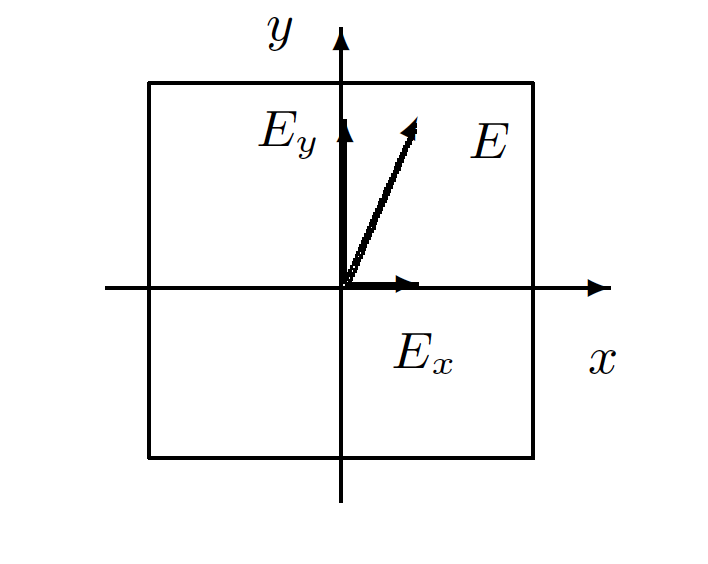
\includegraphics[width=\linewidth]{pics/1.png}
    \caption{Разложение линейно поляризованного света по главным направлениям двоякопреломляющей пластинки}
    \label{pic:1}
\end{wrapfigure}

Эллиптически поляризованный свет можно получить из линейно поляризованного с
помощью двоякопреломляющих кристаллических пластинок.

Двоякопреломляющая пластинка имеет два взаимно перпендикулярных главных
направления, совпадающих с осями эллипсоида диэлектрической проницаемости.
Волны, поляризованные вдоль главных направлений, распространяются в пластинке с
разными скоростями, не изменяя характера своей поляризации. Эти волны
называются главными. Мы будем обозначать показатели преломления для главных
волн через $ n_x $ и $ n_y $, где $ x $ и $ y $ --- главные направления
кристаллической пластинки (рис. 1).

Пусть на пластинку падает линейно поляризованная волна, электрический вектор
которой ориентирован под некоторым углом $ \alpha $ к оси $ x $. Разложим
вектор $ \mathbf{E} $ на составляющие $ E_x $ и $ E_y $. На входе пластинки $
    E_x $ и $ E_y $ находятся в фазе. На выходе из-за разности скоростей между ними
появляется разность хода $ d(n_x - n_y) $, при этом сдвиг фаз определяется
соотношением

\begin{equation}\label{}
    \Delta \phi =  \dfrac{2\pi}{m} = k d(n_x - n_y)
\end{equation}

Как уже отмечалось, при сложении двух взаимно перпендикулярных колебаний,
обладающих некоторым сдвигом фаз, образуется колебание, поляризованное по
эллипсу.

\begin{wrapfigure}{l}{0.25\linewidth}
    \vspace{0mm}
    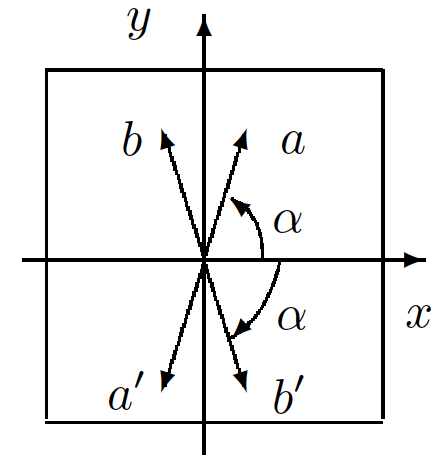
\includegraphics[width=\linewidth]{pics/2.png}
    \caption{Поворот направления колебаний с помощью пластинки в $ \lambda / 2 $}
    \label{ris 2}
\end{wrapfigure}
Рассмотрим практически важные частные случаи.
\begin{enumerate}
    \item Пластинка даёт сдвиг фаз $ 2\pi $ (пластинка в длину волны $ \lambda $). В
          результате сложения волн на выходе пластинки образует- ся линейно
          поляризованная волна с тем же направлением колебаний, что и в падающей волне.
    \item Пластинка даёт сдвиг фаз $ \pi $ (пластинка в полдлины волны $ \lambda / 2 $).
          На выходе пластинки снова образуется линейно поляризованная волна. Направление
          $ bb' $ колебаний этой волны повёрнуто относительно направления $ aa' $
          колебаний падающей волны (рис. 2). Как нетрудно сообразить, направление $ bb' $
          является зеркальным отображением направления $ aa' $ относительно одного из
          главных направлений пластинки. Такую пластинку используют для поворота
          направления колебаний линейно поляризованного света.
    \item Пластинка создаёт между колебаниями сдвиг фаз $ \pi/2 $ (пластинка в четверть
          длины волны). При сложении двух взаимно перпендикулярных колебаний, имеющих
          разность фаз $ \pi/2 $, образуется эллипс, главные оси которого совпадают с
          координатными осями $ x $ и $ y $. При равенстве амплитуд возникает круговая
          поляризация.
\end{enumerate}

Следует отметить, что, говоря о пластинках $ \lambda , \lambda/2, \lambda/4 $ и
т.д., всегда подразумевают какую-либо вполне определённую монохроматическую
компоненту (например, пластинка $ \lambda/2 $ для зелёного света). Если на
двоякопреломляющую пластинку падает не монохроматический свет, то на выходе из
неё для разных спектральных компонент эллипсы поляризации будут различными.

\subsection{Анализ эллиптически поляризованного света}

Анализ эллиптически поляризованного света сводится к нахождению главных осей
эллипса поляризации и к определению направления вращения электрического
вектора.

Главные оси эллипса поляризации определяются с помощью анализатора по максимуму
и минимуму интенсивности проходящего света. Направление вращения электрического
вектора может быть найдено с помощью пластинки в четверть длины волны, для
которой известно, какая из главных волн, $ E_x $ или $ E_y $, имеет б\'{o}льшую
скорость распространения (и соответственно меньшее значение показателя
преломления).

Выберем для определённости координатные оси x и y на пластинке так, чтобы
$n_x<n_y$. В этом случае главная волна $E_x$ имеет большую скорость
распространения. Поместим такую пластинку на пути эллиптически поляризованного
света и совместим главные направления пластинки $ \lambda/4 $ с главными осями
эллипса поляризации. На выходе из этой пластинки сдвиг фаз между $E_x$ и $E_y$
вместо $\pi/2$ станет равным нулю или $\pi$. Свет окажется линейно
поляризованным. Из двух возможных значений сдвига фаз, $0$ или $\pi$,
реализуется одно: то, которое соответствует имеющемуся в волне направлению
вращения электрического вектора.

Рассмотрим, например, случай, когда электрический вектор в эллиптически
поляризованной волне вращается против часовой стрелки, если смотреть навстречу
лучу. В этом случае, очевидно, в волне, падающей на пластинку в $\lambda/4$,
колебание $E_y$ отстаёт по фазе на $\pi/2$ от колебания $E_x$. При прохождении
через пластинку разность фаз увеличивается до $\pi$. Таким образом на выходе из
пластинки возникают линейно поляризованные волны со сдвигом фаз $\pi$. Сложение
этих волн даёт плоскополяризованную волну, электрический вектор которой
располагается во втором и четвёртом квадрантах координатной системы $x$, $y$.

Рассуждая аналогичным образом, найдём, что при вращении электрического вектора
по часовой стрелке направление колебаний в линейно поляризованной волне,
выходящей из пластинки, располагается в первом и третьем квадрантах. Определяя
направление колебаний на выходе из пластинки с помощью поляроида, можно, таким
образом, определить характер эллиптической поляризации (вращение против или по
часовой стрелке).

\subsection{Пластинка чувствительного оттенка}

\begin{wrapfigure}{l}{0.35\linewidth}
    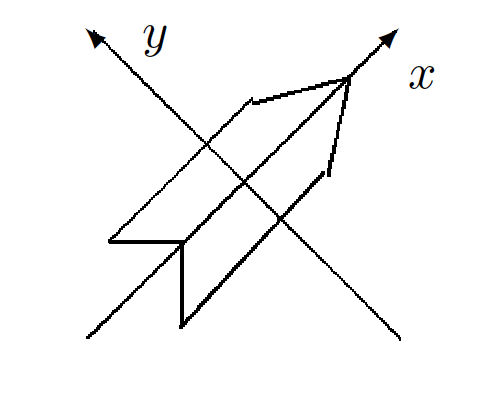
\includegraphics[width=\linewidth]{pics/3.png}
    \caption{Пластинка
        чувствительного
        оттенка}
    \label{ris 3}
\end{wrapfigure}

Выше предполагалось известным, какому из двух главных направлений пластинки в
четверть длины волны соответствует большая скорость распространения света.
Установить это можно различными способами, например с помощью пластинки
чувствительного оттенка (так называют пластинку в $ \lambda $ для зелёной
спектральной компоненты, $ \lambda = 560 $ нм).

Пластинка имеет форму стрелы (рис. 3), вдоль оси которой расположено главное
направление, соответствующее большей скорости распространения.

Если пластинка чувствительного оттенка помещена между скрещенными поляроидами и
главные направления пластинки не параллельны направлениям разрешённых колебаний
поляроидов, то при освещении белым светом пластинка кажется окрашенной в
лилово-красный цвет. Это объясняется тем, что зелёная компонента линейно
поляризованного света при прохождении пластинки не меняет поляризации и
задерживается вторым поляроидом. Для красной и фиолетовой компонент пластинка
создаёт сдвиг фаз, несколько отличный от $ 2\pi $. На выходе из пластинки
красная и фиолетовая компоненты оказываются поэтому эллиптически
поляризованными и частично проходят через второй поляроид. Таким образом, в
известном смысле наблюдаемый в указанном опыте цвет пластинки дополнителен к
зелёному.

Если между скрещенными поляроидами поместить пластинку чувствительного оттенка
($ \lambda $) и пластинку в $ \lambda/4 $ так, чтобы их главные направления
совпадали, цвет пластинки изменится. Если у пластинки чувствительного оттенка и
пластинки в $ \lambda/4 $совпадут главные направления, соответствующие большей
скорости распространения, то разность хода между $ E_x $ и $ E_y $ для зелёного
света составит уже $ 5\lambda/4 $. Это соответствует разности хода в $ \lambda
$ для света с большей длиной волны, т. е. для "<более красного"> света. При
освещении этих пластинок белым светом теперь погасится не зелёная, а красная
часть спектра, и проходящий свет будет казаться зеленовато-голубым. Если же
главные направления, соответствующие большей скорости распространения, у
пластинки чувствительного оттенка и у пластинки в $ \lambda/4 $ окажутся
перпендикулярными, то проходящий свет приобретёт оранжево-желтую окраску
(погасится фиолетово-голубая часть спектра).

Изменение цвета позволяет, таким образом, определить, какое из главных
направлений пластинки в $ \lambda/4 $ соответствует большей скорости
распространения.

\newpage
\subsection{Интерференция поляризованных лучей}

\begin{wrapfigure}{r}{0.35\linewidth}
    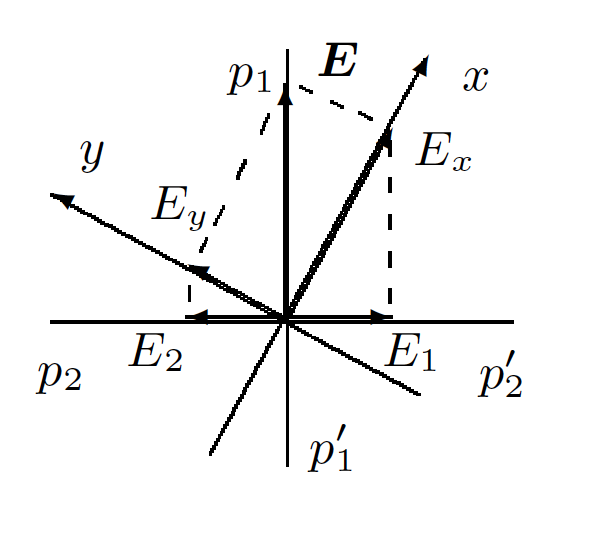
\includegraphics[width=\linewidth]{pics/4.png}
    \caption{К объяснению интерференции поляризованных лучей}
    \label{ris 4}
\end{wrapfigure}

Тонкие двоякопреломляющие пластинки, помещённые между поляроидами, кажутся
окрашенными. Эта окраска может быть истолкована как результат интерференции
поляризованных лучей. На рис. 4 представлена схема для случая скрещенных
поляроидов.

Здесь $ p_1 p'_1 $ --- разрешённое направление колебаний поляризатора (первого
поляроида); $x$, $y$ --- координатная система, связанная с главны- ми
направлениями двоякопреломляющей пластинки; $ p_2 p'_2 $ --- разрешённое
направление колебаний анализатора (второго поляроида). Волны $ E_x $ и $ E_y $
на выходе из пластинки когерентны, но не могут интерферировать, так как $ E_x
    \perp E_y $. Волны $ E_1 $ и $ E_2 $ на выходе второго поляроида также являются
когерентными и к тому же поляризованы в одной плоскости. Эти волны
интерферируют между собой. Результат интерференции определяется зависящим от
длины волны сдвигом фаз между $ E_1 $ и $ E_2 $. В результате интерференции
поляризованных лучей пластинка, освещаемая белым светом, кажется окрашенной.

Если поворачивать двоякопреломляющую пластинку, расположенную между скрещенными
поляроидами, то соотношение амплитуд волн $ E_1 $ и $ E_2 $ и разность фаз
между ними не изменяются. Это означает, что цвет пластинки при её поворотах не
меняется, а меняется только интенсивность света. За один оборот пластинки
интенсивность четыре раза обращается в нуль --- это происходит при совпадении
главных направлений $ x $ и $ y $ с разрешёнными направлениями колебаний
поляроидов.

Если же двоякопреломляющую пластинку оставить неподвижной, а второй поляроид
повернуть так, чтобы разрешённые направления $ p_1p'_1 $ и $ p_2p'_2 $ совпали,
то волны $ E_1 $ и $ E_2 $ приобретают дополнительный фазовый сдвиг на $ \pi $
для всех спектральных компонент; при этом их амплитуды изменятся так, что цвет
пластинки изменится на дополнительный.

\section{Методика измерений и результаты}
\subsection{Направления разрешённых плоскостей поляроидов}

\begin{table}[h]
    \centering
    \begin{tabular}{|c|c|c|c|}
        \hline
        \multicolumn{2}{|c|}{\textbf{Поляроид 1}} & \multicolumn{2}{|c|}{\textbf{Поляроид 2}}                                         \\
        \hline
        \textbf{min}                              & \textbf{max}                              & \textbf{min}      & \textbf{max}      \\
        \hline
        $277 \pm 1^\circ$                         & $186 \pm 5^\circ$                         & $130 \pm 1^\circ$ & $41 \pm 5^\circ$  \\
        \hline
        $97 \pm 1^\circ$                          & $5 \pm 5^\circ$                           & $310 \pm 1^\circ$ & $221 \pm 5^\circ$ \\
        \hline
    \end{tabular}
    \caption{Измерения положений поляроидов, соответвующих минимумам и максимумам интенсивностей пропущенного света}
\end{table}

Если плоскость разрешённого направления направлена под углом $\alpha \in
    [-90,+90]^\circ$, то $\alpha$, $\alpha+180^\circ$ -- положения максимумов;
$\alpha+90^\circ$, $\alpha+270^\circ$ -- положения минимумов.

Тогда $\alpha_1 = (7\pm2)^\circ$, $\alpha_2 = (40\pm2)^\circ$. Будем
использовать эти значения при дальнейшей установке на оптическую скамью.

\subsection{Измерение коэффициента преломления эбонита}
Повторим измерения предыдущего пункта, только для непрозрачного эбонита. Будем
вести наблюдения одним глазом и двигать головой в направлении, перпендикулярном
отражённому лучу -- так легко будет увидеть, когда именно отражение в случае
минимальной интенсивности лежит в центре зеркала, полученный угол отражения от
нормали -- $52^\circ$, при этом заметно, что при отклонении на
$1^\circ$-$2^\circ$ отражение в нужный момент уже не попадает в центр зеркала.
Тогда получим $n = \tan \theta_\text{Б} = (1.28\pm0.05)$.

\subsection{Стопа Столетова}
Будем на свет, прошедший через наклонённые под некоторым углом к лучу пластины.
Вращая поляризатор, заметим, что свет почти линейно поляризован при прохождении
системы пластин. Найдя угол Брюстера, сможем наблюдать подобное уже и в
отражённом свете.

\subsection{Определения главных осей двулучепреломляющих пластин}
Расположим каждую из двулучепреломляющих пластин по очереди между двумя
скрещенными поляризаторами. При повороте у обеих пластин по четыре раза за
оборот достигался минимум интенсивности прошедшего света. Он соотвествовал
совпадению главных осей пластин с разрешенными направлениями поляроидов.

Теперь условно обозначим пластинки как первую и вторую. По очереди расположим
их с первым поляроидом так, что их главные оси составляют угол $45^\circ$ с
поляризатором. Будем вращать второй поляроид-анализатор и наблюдать за
результатом.

В случае первой пластинки интенсивность при повороте анализатора почти не
меняется, что означает, что свет имеет круговую поляризацию. В случае второй же
пластинки отчетливо заметны минимумы и максимумы интенсивности, что означает,
что свет имеет линейную поляризацию.

Таким образом, первая пластинка -- это $\lambda/4$ пластинка, а вторая --
$\lambda/2$.

\subsection{Определение быстрой и медленной оси в пластинке $\lambda/4$}
\begin{wrapfigure}{r}{0.35\linewidth}
    \vspace{-8mm}
    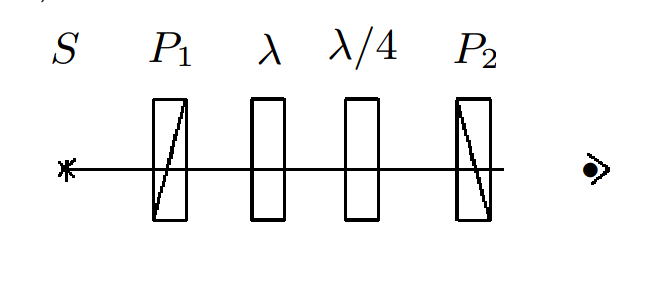
\includegraphics[width=\linewidth]{pics/lambda_4.png}
    \caption{Определение быстрой и медленной оси}
    \label{pic:axes}
\end{wrapfigure}
Рассмотрим анизотропную пластинку чувствительного оттенка (пластинка $\lambda$),
помещённую между скрещенными поляроидами. Прошедший свет окрашен в пурпурный свет:
это объясняется тем, что пластинка не меняет поляризации на той длине волны, для
которой она сделана (зеленый свет, $\lambda_0\approx 560~\mathrm{nm}$). При этом
для компонент ближе к краю оптического диапазона (красный и фиолетовый) пластинка
ведёт себя уже фактически как пластинка, обеспечивающая сдвиг фаз равный
$2\pi \lambda_0 / \lambda$. Это значит, что пластинка меняет для них поляризацию,
и данные компоненты можно увидеть при прохождении через анализатор.

Добавим пластинку $\lambda/4$ к пластинке чувствительного оттенка так, чтобы
направления их главных осей совпали (с точностью до поворота на $90^\circ$).
Если направления быстрой и медленной осей совпадают, то пластинка обеспечивает
сдвиг фаз $\frac{5}{2}\pi \frac{\lambda_0}{\lambda}$, а если нет --
$\frac{3}{2}\pi \frac{\lambda_0}{\lambda}$. Легко вывести формулу, которая
покажет, что спектральная интенсивность пропущенного света пропорциональна
$\sin^2 \left(\frac{z \cdot \pi \lambda_0}{\lambda}\right)$, где $z=(1\pm \frac
    1 4)$. С её помощью вычислим теоретический спектр, и, используя библиотеку
\textit{colour-science}, получим теоретические цвета.

\begin{figure}[H]
    \begin{minipage}[t]{0.48\textwidth}
        \centering
        
\includegraphics[width=0.5\linewidth]{pics/perpendicular.png} % Замените на свой файл
        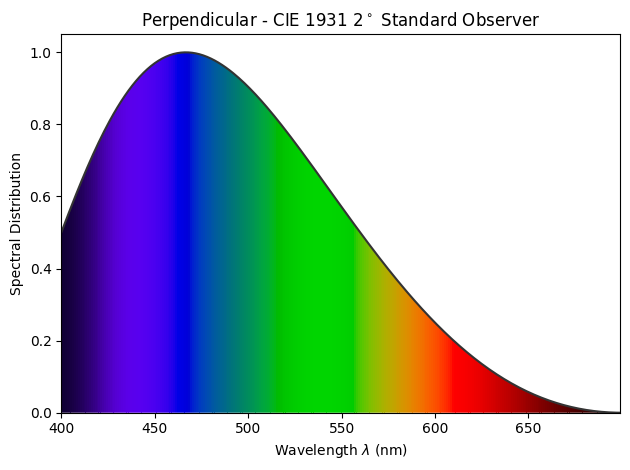
\includegraphics[width=\linewidth]{pics/perpendicular_spectrum.png}
        Cовпадающие направления главных осей
    \end{minipage}
    \hfill
    \begin{minipage}[t]{0.48\textwidth}
        \centering
        
\includegraphics[width=0.5\linewidth]{pics/parallel.png} % Замените на свой файл
        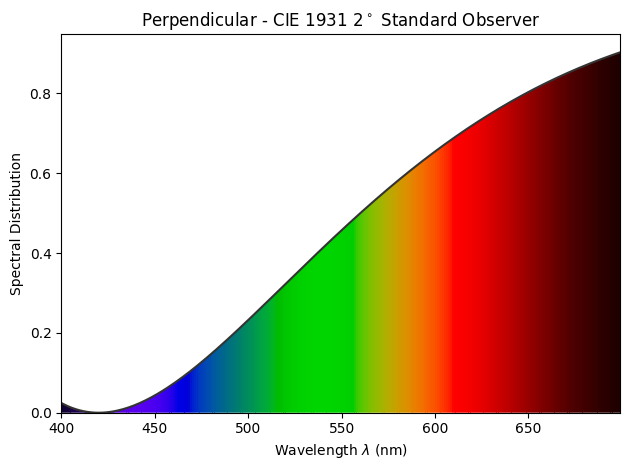
\includegraphics[width=\linewidth]{pics/parallel_spectrum.png}
        Несовпадающие направления главных осей
    \end{minipage}
    \caption{Теоретические спектры и цвета для эксперимента}
    \label{fig:combined}
\end{figure}

И действительно, при повороте эксперимента цвет меняется от красно-оранжевого
до голубо-зелёного. Таким образом, определяем медленную и быструю оси в
пластинке $\lambda/4$.

\subsection{Мозаичная пластинка}
Теперь расположим между скрещенными поляризаторами мозаичную пластинку
\begin{figure}[H]
    \centering % Центрирование всей конструкции
    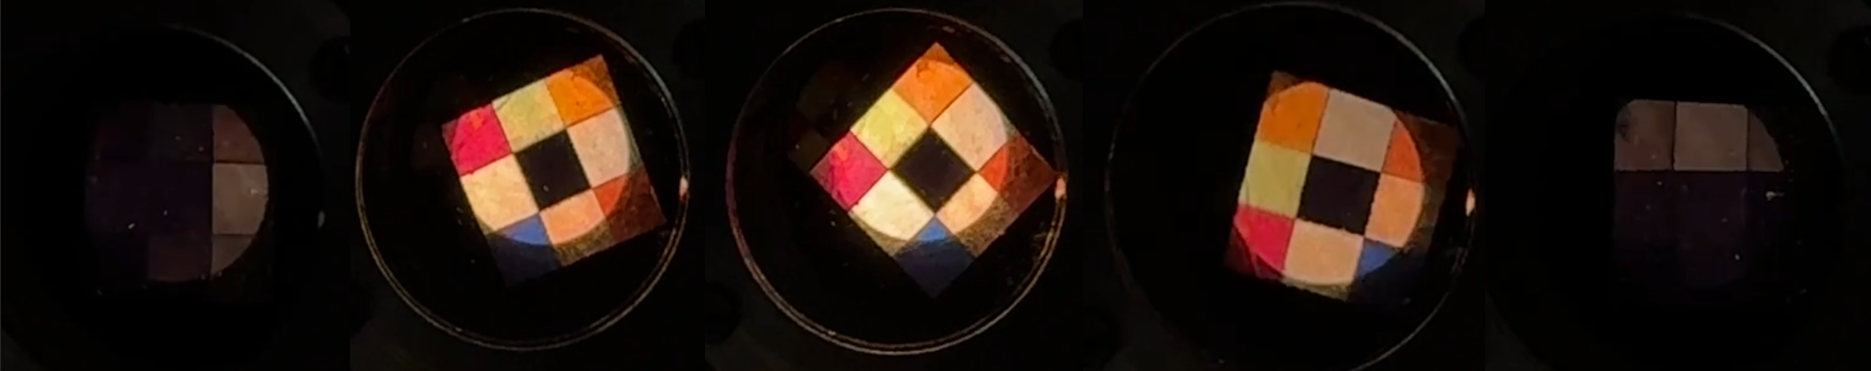
\includegraphics[width=0.6\linewidth]{pics/plate.png}
    \caption{Результат вращения пластинки, смещение -- $45^\circ$}
    \label{pic:plate}
\end{figure}
\begin{figure}[H]
    \centering % Центрирование всей конструкции
    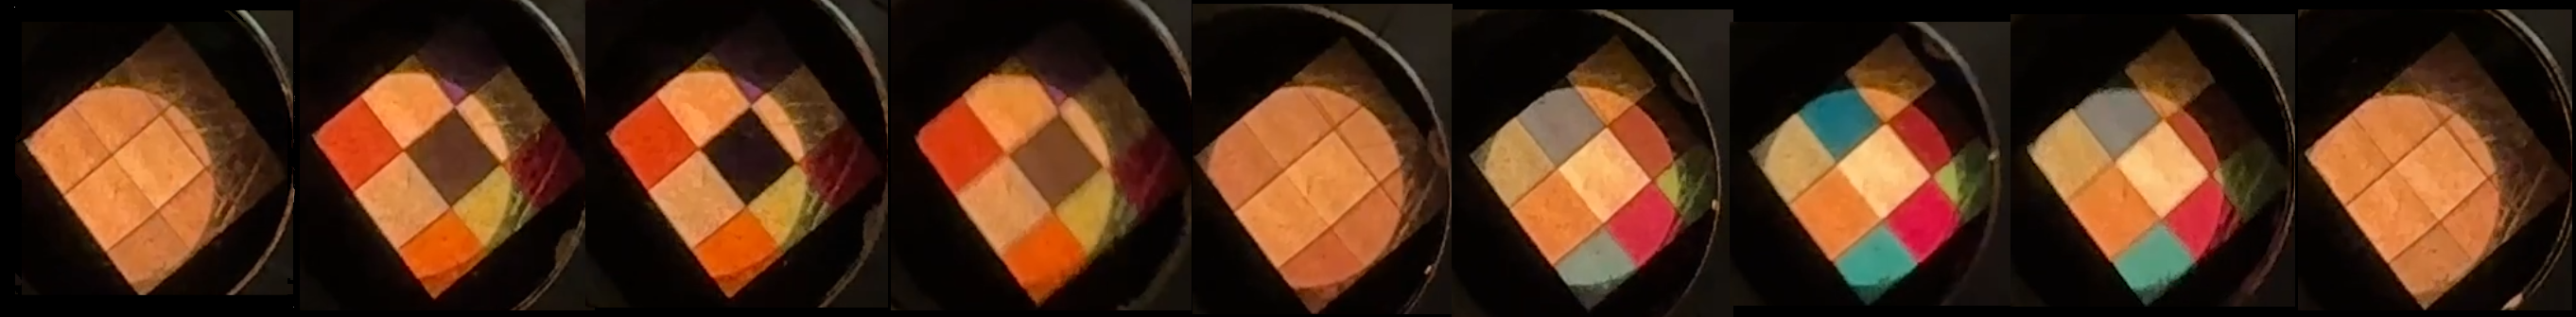
\includegraphics[width=0.95\linewidth]{pics/polaroid.png}
    \caption{Результат вращения поляроида, смещение -- $22.5^\circ$}
    \label{pic:polaroid}
\end{figure}

C учётом того, что одновременно явно наблюдается больше 5 цветов, мы можем
делать лишь какие-то приблизительные догадки. Тем не менее, можно определить
конфигурацию пластинок. Направления всех их быстрых осей совпадают, и
расположены они (ориентируясь на рис. \ref{pic:polaroid}):

\begin{figure}[H]
    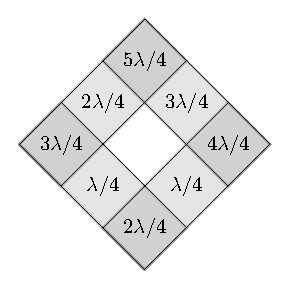
\includegraphics[width=0.4\linewidth]{plates.pdf}
    \caption{Конфигурация пластинок}
    \label{fig:plates}
\end{figure}

\subsection{Определение направления вращения в эллиптически поляризованной
    волне}
Получим эллиптически-поляризованный свет. Для этого установим разрешённое
направление первого поляроида под углом 10–20◦ к горизонтали так, чтобы вектор
$\mathbf{E}$ падающего на пластинку света был расположен в первом квадранте.
Установим разрешённое направление второго поляроида вертикально и, вращая
пластинку, найдём минимальную интенсивность света, прошедшего второй поляроид.
Так получен эллипс поляризации с вертикально ориентированной малой осью.

Для определения направления вращения светового вектора установим между
поляроидами дополнительную пластинку $\lambda/4$ с горизонтально
ориентированной «быстрой» осью. В этом случае свет на выходе из второй
пластинки будет линейно поляризован. Если пластинки поодиночке дают эллипсы,
вращающиеся в разные стороны, то поставленные друг за другом, они скомпенсируют
разность фаз, и вектор E на выходе останется в первом и третьем квадрантах.
Если же световой вектор перешёл в смежные квадранты, значит, эллипсы вращаются
в одну сторону.

В итоге получим, что свет на выходе из первой пластинки имеет правую
поляризацию, так как плоскость поляризации перешла в смежный квадрант.

\section{Вывод}
В результате работы мы изучили некоторые эффекты, связанные с поляризацией
света, а именно поляризацию при отражении и прохождении через границу сред, а
также влияние двоякопреломляющих пластинок на поляризацию света. По цвету и
интенсивности прошедшего освещения оказалось возможным определить параметры
двоякопреломляющих пластин, такие как направление главных осей и их
<<номинальный>> сдвиг фаз по осям.
\end{document}
